\documentclass{article}
\usepackage[utf8]{inputenc}
\usepackage{tabularx}
\usepackage{booktabs}
\usepackage{hyperref}
\usepackage{listings}
\usepackage{fancyvrb}
\usepackage{graphicx}
\usepackage[citestyle=numeric,bibstyle=numeric]{biblatex}
\graphicspath{ {./images/} }

\addbibresource{bibliography.bib}

\VerbatimFootnotes{}


%Style
\usepackage{xcolor}
 
\definecolor{codegreen}{rgb}{0,0.6,0}
\definecolor{codegray}{rgb}{0.5,0.5,0.5}
\definecolor{codepurple}{rgb}{0.58,0,0.82}
\definecolor{backcolour}{rgb}{0.95,0.95,0.92}
 
\lstdefinestyle{mystyle}{
    backgroundcolor=\color{backcolour},   
    commentstyle=\color{codegreen},
    keywordstyle=\color{magenta},
    numberstyle=\tiny\color{codegray},
    stringstyle=\color{codepurple},
    basicstyle=\ttfamily\footnotesize,
    breakatwhitespace=false,         
    breaklines=true,                 
    captionpos=b,                    
    keepspaces=true,                 
    numbers=left,                    
    numbersep=5pt,                  
    showspaces=false,                
    showstringspaces=false,
    showtabs=false,                  
    tabsize=2
}
 
\lstset{style=mystyle}
%Style

\newcommand{\qq}[1]{``#1''}

\setlength{\parindent}{0pt}
\setcounter{section}{-1}

\title{Python Tutorial}
\author{Dominique Hansen}
\date{\today}

\begin{document}

\maketitle

\section{Getting Started}

\subsection{Installing Python}

\subsubsection{Linux}\label{linux_python_install}
Many linux systems have Python already installed.
Older systems might have Python2 alongside Python3.
Refrain from using Python2 since it is not fully compatible with Python3
and reached its end of life with the start of 2020.

On debian based systems Python3 can be installed with apt in the terminal:

\begin{lstlisting}[language=Bash]
sudo apt-get install python3.8
# Or just 3 if 3.8 is not available for you
sudo apt-get install python3
\end{lstlisting}

\subsubsection{Windows 10}
Windows 10 supports running linux inside itself with the
``Windows Subsystem for Linux''.\footnote{\href{https://docs.microsoft.com/en-us/windows/wsl/install-win10}{Installation Guide}}
If you choose a debian based subsystem like ubuntu, you can use the
installation command from the section{~}\ref{linux_python_install}.

\subsection{Windows 7}
If you still have a Windows 7 installion on your personal PC you should upgrade to Windows 10.
Windows 7 is no longer save to work in.
If you have to work with a Windows 7 systems on your work station at the DIW you can use conda.
You can get an installer for anaconda \href{https://www.anaconda.com/distribution/#download-section}{here}.
Anaconda can be installed without Admin privileges if you only install it for your user.
Install the full anaconda distribution not miniconda.




\subsection{Your Development Environment}

Probably the most popular editors for python developers are
\href{https://code.visualstudio.com/}{Visual Studio Code}
and \href{https://www.jetbrains.com/pycharm/}{PyCharm}.
PyCharm is specifically geared towards development in Python.
VSCode was created for web development but it also has a wide array of
extensions that allow you to work with other languages.
The Python extension is very mature and actively developed by microsoft.
VSCode is completely open source whereas PyCharm is partially open source, with
a free and a commercial version.

\subsubsection{VSCode Setup}

Get an installer for your system at
\href{https://code.visualstudio.com/}{code.visualstudio.com}.
Once installed open VSCode and install the Python extension.
\begin{itemize}
    \item Extensions can be opened via the toolbar on the left or with Ctrl+Shift+x.
    \item Search for Python in the extensions, first result should be the correct one.
    \item Open settings. Shortcut here is Ctrl+,
    \item On Windows search the settings for the entry
          ``Python: Conda Path'' and set it for your system.\footnote{Will Probably be at\\ \
              \verb!D:\Users\YOURUSERNAME\AppData\Local\Continuum\anaconda3\Scripts\conda.exe! }
    \item Onm Linux the Path to Python will probably already be set correctly.
    \item Enable all linters and style checker, that you like.
    \item VSCode will help you with the installation of linters and style checkers,
          if the Python or Conda path ist set correctly.
\end{itemize}

\subsubsection{Linters, Stylecheckers and Formatters}

A Linter is a program, that ``looks'' at your code and warns you about potential
problems with it. These Problems include:
\begin{itemize}
    \item Not adhering to a style guide.
    \item Not adhering to conventions.
    \item Your code contains structures that are commonly associated with errors.
    \item Your code contains structures that make it harder to maintain.
    \item Your code contains actual errors, like syntax errors, that would crash it on execution.
\end{itemize}

Popular linters for Python are \href{https://github.com/PyCQA/pylint}{pylint} and
\href{https://github.com/PyCQA/pyflakes}{pyflakes}.
Pylint is more feature rich than pyflakes.
The amount of things Pylint checks can be overwhelming but the checks can be limited
via configuration files.

A popular linter specialized on code style, a style checker,
is \href{https://github.com/PyCQA/pycodestyle}{pycodestyle}.
It checks if your code adheres to the Python
\href{https://www.python.org/dev/peps/pep-0008/}{PEP 8} style guide.

Many problems such linters might find, can potentially be fixed automatically.
Black is a formatter, that can fix many style guide violations automatically.
It is an opinionated formatter, meaning that it is not very configurable by design.
Black also tries to format your code in a way to improve git diffs.

There is no ``one'' way to format your code.
PEP 8 was developed by people who were highly involved and experienced in Python.
It is however not the be-all and end-all on how to style your code.
Not adhering to it does not make your code ``wrong''.
But it is a piece of shared knowledge between many Python programmers.
Adhering to and knowing the conventions makes it easier for you to understand
the code of others and your own code after you did not look at it for a long time.

\section{Python compared to other languages}

\subsection{Python compared to R}

\begin{table}[h]
    \begin{tabularx}{\linewidth}{>{\parskip1ex}X@{\kern4\tabcolsep}>{\parskip1ex}X}
        \toprule
        \hfil\bfseries Python
         &
        \hfil\bfseries R
        \\\cmidrule(r{3\tabcolsep}){1-1}\cmidrule(l{-\tabcolsep}){2-2}

        %% PROS, seperated by empty line or \par
        Was deveoped as teaching tool for programming.

        Is a general purpose scripting language.

        Is itself programmed in C and Python.

        Main package repository is \href{https://pypi.org/}{pypi} with 216.195 packages.

        Has a \href{https://github.com/mre/awesome-static-analysis\#python}{large library}
        of software that helps developers write good code.

        Has \href{https://www.python.org/dev/peps/pep-0008/}{official best practices}
        to help in writing more comprehensible code.

        Has a unittesting library in its own standard library.

         &

        %% CONS, seperated by empty line or \par
        Was developed by statisticians for statisticians.

        Is a domain specific scripting language.

        Is itself programmed in C, Fortran and R.

        Main package repository is \href{https://cran.r-project.org/}{CRAN} with 15.330 packages.

        Has a \href{https://github.com/mre/awesome-static-analysis\#r}{small library}
        of software that helps developers write good code.

        Has no consensus on style or best practices.

        Has third party libraries for unittesting.

        \\\bottomrule
    \end{tabularx}
\end{table}

\section{Pythonsyntax}

Most languages use visible characters to define a
\href{https://en.wikipedia.org/wiki/Block_(programming)}{code block}.

A loop in R can look like this:

\begin{lstlisting}[language=R]
for(number in 1:10) {
print(number)
}
\end{lstlisting}

And the same loop can also look like this:

\begin{lstlisting}[language=R]
for(number in 1:10){print(number)}
\end{lstlisting}

Or like this:

\begin{lstlisting}[language=R]
for(number in 1:10) {
    print(number)
}
\end{lstlisting}


The whitespace in the third example carries no syntactical meaning.
But similar indention is used by many programmers to make their
code more readable.
It makes it easier for people to determine the block a line of code belongs to.
Python on the other hand uses whitespace explicitly to denote a block.
The same loop in python would look like this:

\begin{lstlisting}[language=Python]
for number in range(1, 11):
    print(number)
\end{lstlisting}

Python forces its users to write cleaner looking code through its use of whitespace
as syntactical characters.
As a teaching language it was created with readability of the code in mind.

Python does not care if you use spaces or tab characters as long as it is consistent.
It is also not relevant for Python how many spaces or tabs are used as long as it is consistent.
As with many scripting languages Python leaves some freedom to its users.
It is however strongly recommended\footnote{
    Python has a Style Guide
    \href{https://www.python.org/dev/peps/pep-0008/}{PEP 8}
}
to use only spaces and keep the number of spaces to exactly 4.
Adhering to the style guide makes it easier for others (yourself in the future included)
to reuse the code.


\section{Statements and Expressions}

An expression is a portion of code, that evaluates to a value.
Expressions can be combined to form new expressions.
\begin{lstlisting}[language=Python]
1 + 2 # This is an expression.
4 * 5 # This is another expression.
1 + 2 + 4 * 5 # This is still an expression.
some_function() # This is also an expression.
1 < 2 # This is the last expression.
\end{lstlisting}

A statement is a line of code that causes an action to be performed.
The above expressions are also statements in Python, since they .
The action that is performed there, is the evaluation of the respective expression.
Statements can not be combined to form new statements.

\begin{lstlisting}[language=Python]
import os # This is a statement.
x = 1 # This is a statement.
y = 1 + 2 # This is a statement.
if y==3: # This is a statement.
    z = some_function() # This is a statement. 
y = x = 1 + 2 # This is incorrect python syntax.
\end{lstlisting}


\section{Decisions and Loops}

\subsection{if, elif, else}

Decision making is an important part in most programms.
Oftentimes we have to handle data differently depending on
the makeup of the data.
Or we have to decide to do certain things if our data is a certain way.

To do this we can make use of the $if$, $if\cdots else$ and $if\cdots elif$
statements:

\begin{lstlisting}[language=Python]
if a_variable == 1:
    print("It is one.")
elif a_variable == 2:
    print("It is two.")
else:
    print("That's too much, man!")
\end{lstlisting}

If the statement at $if$ evaluates to True ``This is one.'' will be printed.
If it evaluates to False, the $elif$ statement is checked.
An $if$ statement can be followed by an arbitrary amount of $elif$ statements.
Only the one that evaluates to True gets its block executed, all statements
after that will be skipped.
The $else$ block will only be executed if all other checks evaluate to False.

\subsubsection{What is True?}

Obviously boolean $True$ and $False$ values evaluate to what they say.
But in python there are also ``Truthy'' and ``Falsy'' values.
These values are not of the type boolean but will be treated as such in the right context:

\begin{lstlisting}[language=Python]
a_list = []

if a_list:
    print("The first element is: " + a_list[0])
else:
    print("The list is empty.")
\end{lstlisting}

\begin{itemize}
    \item An empty list, dictionary, set, string or a 0 will evaluate to False in a boolean context.
    \item The special $None$ value will also evaluate to False.
    \item A list, dictionary or set with at least one element will evaluate to True.
    \item All numbers other than 0 and a string with at least one character will also evaluate to True.
\end{itemize}






\section{Data Types, Sequences, Sets and Dictionaries}

The type of a variable is determined by the Python interpreter at the time
of execution.
The interpreter can convert values to different types when it is necessary.

\subsection{Build-in Types}

Python has extensive \href{https://docs.python.org/3/library/stdtypes.html}{documentation}
on their build-in types.
The most basic types, which you will most commonly handle are:

\begin{itemize}
    \item integer
    \item float
    \item boolean
    \item string
\end{itemize}

These are immutable, i.e.\@ their value cannot be changed.
Operations performed on them always create a completely new ``thing''.
Their counterpart are mutable types, which can be changed.

\subsubsection{Problems with numbers}

Due to the way computers work there are two main sources of error, when working
with numbers.
The first is overflow.
This happens when a number reaches the upper or lower limit of the numberrange
that can be presented in memory by a language.
If you add 1 to the highest possible number, the number overflows and wraps around
into the negativ range to the lowest possible number.
Same happens in reverse if you take away 1 from the lowest possible number.

The way Python3 is build, this is not a problem for integers.
Python integers can be of arbitrary size.
It is however a problem for float numbers and can be in packages like pandas
and numpy, since they use the underlying C integer type directly.

The other problem is the precision of floating point numbers.
Not all decimal numbers can be accurately represented in a computer.


\begin{lstlisting}[title={Precision error in Python}]
>>> 0.1 + 0.2 == 0.3
False
>>> 0.1 + 0.2
0.30000000000000004
>>> 0.1 + 0.2 - 0.3
5.551115123125783e-17
\end{lstlisting}

\begin{lstlisting}[title={Precision error in R}]
> 0.1 + 0.2 == 0.3
[1] FALSE
> 0.1 + 0.2
[1] 0.3
> 0.1 + 0.2 - 0.3
[1] 5.551115e-17
\end{lstlisting}

As you can see on the R example, languages sometimes hide these errors in their
output by rounding.
For most purposes these errors are so small as to be deemed negligible.
But they can add up when performing large many consecutive calculations.
You should keep this in mind if you need high precision in your calculations.
There may be libraries you can use that can perform calculations with higher
precision.


%http://pythontutor.com/visualize.html#code=NUMBER%20%3D%202%0AADD_RESULT%20%3D%20NUMBER%20%2B%202%0ADIV_RESULT%20%3D%20ADD_RESULT%20/%20NUMBER%0AMULT_RESULT%20%3D%20DIV_RESULT%20*%203%0AMODULO_RESULT%20%3D%20%28MULT_RESULT%20%2B%201%29%20%25%202%0A_STRING%20%3D%20%22HELLO%20WORLD%22%0A_LIST%20%3D%20list%28%29%0A_LIST2%20%3D%20%5BNUMBER,%20_STRING%5D%0A_LIST.append%28NUMBER%29%0A_LIST.append%28ADD_RESULT%29%0A_LIST.append%28_LIST2%29%0A_LIST2%5B0%5D%20%3D%20ADD_RESULT%0A_TUPLE%20%3D%20%281,2,3%29%0A_LIST%5B2%5D%20%3D%20_TUPLE%0A_TUPLE%20%3D%20_TUPLE%20%2B%20_TUPLE%0A_LIST%5B2%5D%20%3D%20_LIST2%0A_LIST2%20%3D%20_LIST2.append%28_LIST2%29&cumulative=false&curInstr=17&heapPrimitives=nevernest&mode=display&origin=opt-frontend.js&py=3&rawInputLstJSON=%5B%5D&textReferences=false

\subsection{Lists}\label{lists}

As the name suggests, this is a list of ``things''.
It can contain everything that can also be assigned to a variable.
Lists are mutable. They can be changed.
Elements can be added or removed from a list after it has been created.

Lists can be created empty:

\begin{lstlisting}[language=Python]
an_empty_list = list()
another_empty_list = []
\end{lstlisting}

and then be filled:

\begin{lstlisting}[language=Python]
list_for_content = an_empty_list
list_for_content.append(1)
# The name of an_empty_list is now a lie.
list_for_content.append(2)
list_for_content.append(3)
\end{lstlisting}

It can also be created with content:

\begin{lstlisting}[language=Python]
a_list_with_content = [1 ,2 ,3]
\end{lstlisting}

Elements of a list can be accessed like this:

\begin{lstlisting}[language=Python]
a_list_with_content[0]
a_list_with_content[2]
\end{lstlisting}

Indices in Python start at 0, meaning that
$an\_empty\_list[0]$ will be $1$ and $an\_empty\_list[2]$
will be 3.

\href{http://pythontutor.com/visualize.html\#code=an\_empty\_list\%20\%3D\%20list\%28\%29\%0Aanother\_empty\_list\%20\%3D\%20\%5B\%5D\%0A\%0Alist\_for\_content\%20\%3D\%20an\_empty\_list\%0Alist\_for\_content.append\%281\%29\%0A\%23\%20The\%20name\%20of\%20an\_empty\_list\%20is\%20now\%20a\%20lie.\%0Alist\_for\_content.append\%282\%29\%0Alist\_for\_content.append\%283\%29\%0A\%0Aa\_list\_with\_content\%20\%3D\%20\%5B1\%20,2\%20,3\%5D\%0A\%0Aprint\%28an\_empty\_list\%29\%0Aprint\%28another\_empty\_list\%29\%0Aprint\%28list\_for\_content\%29\%0Aprint\%28a\_list\_with\_content\%29\%0A\%0Aprint\%28an\_empty\_list\%5B0\%5D\%29\%0Aprint\%28an\_empty\_list\%5B2\%5D\%29\&cumulative=false\&curInstr=13\&heapPrimitives=nevernest\&mode=display\&origin=opt-frontend.js\&py=3\&rawInputLstJSON=\%5B\%5D\&textReferences=false }
{Here is an executable example.}


\subsubsection{Interlude: Mutability}

As you can see in the executable example, the list, that was supposed to be empty, is no longer empty.
When you pass a mutable object to something else, you do not pass a copy of it.
You pass a reference, which in turn points to the exact same object in the computers memory.

When assigning $an\_empty\_list$ to $list\_for\_content$, $list\_for\_content$ gets assigned
the reference contained in $an\_empty\_list$.
When we added values to $list\_for\_content$, $an\_empty\_list$ also changed, since they
point to the same \textbf{changeable} object inside the computers memory.
The same thing will happen, if you pass a changeable object into a function, that
makes changes on the passed object.
You have to keep this in mind in order not change objects accidentally.

There are ways to work on a copy of an object without changing the original.
Lists and dictionaries\footnote{\ref{dictionary}} have the inbuilt method $copy$
to do that.
Note that this will only copy the lists content into another list.
If the list contains mutable objects, they will not be copied, they will be passed
as reference to the new list.
If you want to be sure not to change anything in the original object you can use
the copy library and make a deepcopy.
You can go through this \href{http://pythontutor.com/visualize.html#code=an_empty_list%20%3D%20list%28%29%0Aanother_empty_list%20%3D%20%5B%5D%0A%0Alist_for_content%20%3D%20an_empty_list.copy%28%29%0Alist_for_content.append%281%29%0A%23%20The%20name%20of%20an_empty_list%20is%20now%20a%20lie.%0Alist_for_content.append%282%29%0Alist_for_content.append%283%29%0A%0Aa_list_with_content%20%3D%20%5B1%20,2%20,3%5D%0A%0Aprint%28an_empty_list%29%0Aprint%28another_empty_list%29%0Aprint%28list_for_content%29%0Aprint%28a_list_with_content%29%0A%0Aprint%28len%28an_empty_list%29%29%0A%0Aimport%20copy%0A%0Aa_list_of_empty_lists%20%3D%20%5B%0A%20%20%20%20an_empty_list,%0A%20%20%20%20another_empty_list%0A%5D%0A%0Aa_list_copy%20%3D%20a_list_of_empty_lists.copy%28%29%0Aa_list_deepcopy%20%3D%20copy.deepcopy%28a_list_of_empty_lists%29%0Aa_list_copy.append%28%5B1,2,3%5D%29%0Aa_list_copy%5B0%5D.append%281%29%20%23%20This%20will%20change%20the%20original%20an_empty_list&cumulative=false&curInstr=15&heapPrimitives=nevernest&mode=display&origin=opt-frontend.js&py=3&rawInputLstJSON=%5B%5D&textReferences=false}
{interactive example} to see how copy and deepcopy work.



%([&%$#_{}~^\\]) \\\\\\1

%http://pythontutor.com/visualize.html#code=an_empty_list%20%3D%20list%28%29%0Aanother_empty_list%20%3D%20%5B%5D%0A%0Alist_for_content%20%3D%20an_empty_list%0Alist_for_content.append%281%29%0A%23%20an_empty_list%20name%20is%20now%20a%20lie%0Alist_for_content.append%282%29%0Alist_for_content.append%283%29%0A%0Aprint%28list_for_content%29%0Aprint%28an_empty_list%29&cumulative=false&curInstr=8&heapPrimitives=nevernest&mode=display&origin=opt-frontend.js&py=3&rawInputLstJSON=%5B%5D&textReferences=false

\subsubsection{Slicing}

Slicing gives you an easy and comprehensible way to get a part of a list.
Slicing a list looks similar to addressing a single element:

\begin{lstlisting}[language=Python]
# The range() function is useful for the creation of numerical sequences.
n_up_to_a_hundred = list(range(1,101))
n_up_to_50 = n_up_to_a_hundred[:50]
multiples_of_two_up_to_50 = n_up_to_a_hundred[1:50:2]
\end{lstlisting}
The numbers between the brackets provide [first index:last index:step]


\subsubsection{List comprehension}

List comprehension, somewhat like slicing, lets us create a list from another list.
Slicing only allows us to select elements from a list by index.
List comprehension is far more powerful.

\subsection{Dictionaries}\label{dictionary}

A dictionary is similar to what is called hash map or hash table in other languages.
It is a collection of values, that can be accessed by keys.
A key can be any value that is immutable.
Similar to a real life dictionary, if you know the name of something, you can look up
information about that thing inside a Python dictionary.
Dictionary values can be accessed like lists with angular braces $[]$.
But instead of passing an index a key is passed to the dictionary.

\begin{lstlisting}[language=Python]
CLASS_AGE = {
    "Anne": 27,
    "John": 25,
    "Marie": 24,
    "Dan": 30,
}

if CLASS_AGE["John"] == 25:
    print("John is 25")
\end{lstlisting}

\href{http://pythontutor.com/visualize.html\#code=CLASS\_AGE\%20\%3D\%20\%7B\%0A\%20\%20\%20\%20\%22Anne\%22\%3A\%2027,\%0A\%20\%20\%20\%20\%22John\%22\%3A\%2025,\%0A\%20\%20\%20\%20\%22Marie\%22\%3A\%2024,\%0A\%20\%20\%20\%20\%22Dan\%22\%3A\%2030,\%0A\%7D\%0A\%0A\%23\%20This\%20is\%20True\%0Aif\%20CLASS\_AGE\%5B\%22John\%22\%5D\%20\%3D\%3D\%2025\%3A\%0A\%20\%20\%20\%20print\%28\%22John\%20is\%2025\%22\%29\%0A\%20\%20\%20\%20\%0Afor\%20key,\%20value\%20in\%20CLASS\_AGE.items\%28\%29\%3A\%0A\%20\%20\%20\%20print\%28f\%22\%7Bkey\%7D\%20is\%20\%7Bvalue\%7D\%20years\%20old.\%22\%29\&cumulative=false\&curInstr=15\&heapPrimitives=nevernest\&mode=display\&origin=opt-frontend.js\&py=3\&rawInputLstJSON=\%5B\%5D\&textReferences=false}
{Interactive example at pythontutor.com}

\subsubsection{Dictionary Comprehension}

Like list comprehension for dictionaries.
Is done in curly brackets like a dictionary declaration.

\begin{lstlisting}[language=Python]
# index % 2 == 1 would be more readable but did not fit on a line.
even_odd_mapping = {
    index: "odd" if index % 2 else "even" for index in range(10)
}
\end{lstlisting}

\subsection{Sets}

A set is a list of values where no duplicates are possible.
If a value is added twice to a set, it is not added to the set again.
This is done through hashing mechanisms.\footnote{
    Called \href{https://en.wikipedia.org/wiki/Hash_function}{hashing}
}
So they function somewhat like a dictionary with only keys.
Like dictionary keys, sets can only contain immutable values.

\subsection{Tuple}

A tuple is a list of values.
It is, in contrast to the normal list type, immutable
Once set, a tuple cannot be changed.
This means that a tuple, that only contain immutable values, can be a dictionary key.

\subsection{Choosing your data structure}

You can accomplish many tasks while just using one of these more complex data structures.
But each has its own pros and cons.
If you want to be create an efficient program, you should think about which data structures
to use.

A common trade of in efficient programming is time vs. space.
A dictionary for example, consumes more space than a list.
If you want to know if a specific value is the dictionaries, you look for
it through its key in a time of $\mathcal{O}(1)$\footnote{Simplified
    $\mathcal{O}$ is used in Computer science to denote runtime.
    As the size of the dictionary approaches infinity the access time will still be 1.
}.
If you want to know the same for a list, for the worst case scenario, you would
have to go through the whole list.
So if the list is n elements long, it would take a time of $\mathcal{O}(n)$.

\section{Functions}

A function is a code structure, that accepts some form of input, does something
and returns a value.
Functions can be used centralize redundant tasks in your code.
Imagine we want to remove even numbers from several lists.
We could do this \qq{by hand} like this:

\begin{lstlisting}[language=python]
some_numbers = [1, 2, 3, 4, 4, 5, 4]
some_more_numbers = [2, 2, 2, 3, 3, 4, 4, 4, 5, 5]

for index, number in enumerate(some_numbers):
    if (number%2==0):
        del some_numbers[index]

for index, number in enumerate(some_more_numbers):
    if (number%2==0):
        del some_more_numbers[index]
\end{lstlisting}

Or we could encapsulate this functionality in a function.

\begin{lstlisting}[language=python]
from typing import List # Typing is optional but highly recommended.

# This would be the basic function statement:
# def remove_even(numbers):
# I would highly recommend type hinting your functions.
def remove_even(numbers: List[int]) -> List[int]:
    """Remove even numbers from a list."""
    cleaned_numbers = list()
    for number in numbers:
        if (number%2==1):
            cleaned_numbers.append(number)
    return cleaned_numbers
    

some_numbers = [1, 2, 3, 4, 4, 5, 4]
some_more_numbers = [2, 2, 2, 3, 3, 4, 4, 4, 5, 5]

some_numbers = remove_even(some_numbers)
some_more_numbers = remove_even(some_more_numbers)
\end{lstlisting}


\section{Iterators and Generators }\label{generators}

\qq{Any object that implements the $\_\_next\_\_$ no-argument method,
    which returns the next item in a series, or raises StopIteration
    when there are no more items}\cite{Ram2015}

This is the formal definition of the iterator design pattern in Python.
You do not have to understand this right now but you can come back to it when
you understand more about Objects.


In simplified terms, an iterator is something that can be iterated on.
It \qq{contains} data and you can ask it for the next piece of data.
Most of the iterators you will work with are probably created implicitly.
When using the $for$ loop on lists for example, it will get an iterator from the
list object and iterate with it.

\begin{lstlisting}[language=Python]
for number in [1, 2, 3, 4]:
    print(number)
\end{lstlisting}

A generator is a type of iterator.
But it does not contain the elements that can be iterated over.
Instead it generates values on the fly.
This saves memory and enables iteration over infinite collections.
You can easily write your own generator by using the $yield$ instead of the
return statement in a function.

\begin{lstlisting}[language=Python]
def fibonacci_numbers() -> int:
    """A generator for all fibonacci_numbers."""
    last_number = 0
    current_number = 1
    yield last_number
    while True:
        current_number, last_number = (current_number + last_number, current_number)
        yield current_number
\end{lstlisting}

Some libraries like pandas also give you options to iterate over data with a
generator.
This makes it possible to work with data, that would not fit in your
systems memory.

\section{Classes and Objects}

A class is a template for objects, that defines preset data and functionality.
In Python3 a class defines a type, meaning that every value is an object,
since it is an instance of a class.
Really Everything in Python3 is an object.
Even basic types like integers and float are objects.
Functions are also objects.

\begin{lstlisting}[language=python]
>>> isinstance(1, object)
True
>>> isinstance(print, object)
True
\end{lstlisting}

But what exactly is an object?
While a class is an the general definition of a class of entities, an object
is a specific instance of an entity.
The terms object and instance are often used interchangeably.
Like the class itself an object combines data and functionality.
Imagine car as a class of entities.
All (function, street legal) cars can accelerate, break and have a horn.

\begin{lstlisting}
class Car():

    horn_sound: str = "Honk!"
    _speed: float = 0.0

    def __init__(self, horn_sound: str = None):
        if horn_sound:
            self.horn_sound = horn_sound

    def accelerate(self, kmh: float = 0.0):
        self._speed = self._speed + kmh

    def brake(self, target_kmh: float = 0.0):
        if target_kmh < self._speed:
            self._speed = float(target_kmh)

    def honk(self):
        print(self.horn_sound)

    @property
    def speed(self):
        return f"{self._speed} km/h"


\end{lstlisting}

Functions that bind to an object are called methods in Python.
The $\_\_init\_\_$ method is called implicitly when the class is called.
It is used to set initial values for an object.
The $\_\_init\_\_$ exists in every class, even if you do not declare it explicitly.
If it is not declared, all the $\_\_init\_\_$ will do is return the instantiated object.
Which it also does implicitly after the execution of your method block,
if you declare it explicitly.
\footnote{The $\_\_init\_\_$ is part of Pythons magic methods,
    also called dunder (double underscore) methods.
    They are a set of methods that provide special functionality.
    If, for example, an object implements the $\_\_add\_\_$ method the $+$ operator
    can be used with it.
    Or you can implement the $\_\_next\_\_$ method to makes an object iterable}

If we want to keep track of several cars we can now do this:

\begin{lstlisting}[language=python]
my_car = Car()
your_car = Car("Biep!")

my_car.accelerate(30)
your_car.accelerate(40)

print(my_car.speed)
print(your_car.speed)

my_car.honk()
your_car.brake(30)
your_car.honk()

print(my_car.speed)
print(your_car.speed)
\end{lstlisting}

\href{http://pythontutor.com/visualize.html#code=class%20Car%28%29%3A%0A%0A%20%20%20%20horn_sound%3A%20str%20%3D%20%22Honk!%22%0A%20%20%20%20_speed%3A%20float%20%3D%200.0%0A%0A%20%20%20%20def%20__init__%28self,%20horn_sound%3A%20str%20%3D%20None%29%3A%0A%20%20%20%20%20%20%20%20if%20horn_sound%3A%0A%20%20%20%20%20%20%20%20%20%20%20%20self.horn_sound%20%3D%20horn_sound%0A%0A%20%20%20%20def%20accelerate%28self,%20kmh%3A%20float%20%3D%200.0%29%3A%0A%20%20%20%20%20%20%20%20self._speed%20%3D%20self._speed%20%2B%20kmh%0A%0A%20%20%20%20def%20brake%28self,%20target_kmh%3A%20float%20%3D%200.0%29%3A%0A%20%20%20%20%20%20%20%20if%20target_kmh%20%3C%20self._speed%3A%0A%20%20%20%20%20%20%20%20%20%20%20%20self._speed%20%3D%20float%28target_kmh%29%0A%0A%20%20%20%20def%20honk%28self%29%3A%0A%20%20%20%20%20%20%20%20print%28self.horn_sound%29%0A%0A%20%20%20%20%40property%0A%20%20%20%20def%20speed%28self%29%3A%0A%20%20%20%20%20%20%20%20return%20f%22%7Bself._speed%7D%20km/h%22%0A%20%20%20%20%20%20%20%20%0Amy_car%20%3D%20Car%28%29%0Ayour_car%20%3D%20Car%28%22Biep!%22%29%0A%0Amy_car.accelerate%2830%29%0Ayour_car.accelerate%2840%29%0A%0Aprint%28my_car.speed%29%0Aprint%28your_car.speed%29%0A%0Amy_car.honk%28%29%0Ayour_car.brake%2830%29%0Ayour_car.honk%28%29%0A%0Aprint%28my_car.speed%29%0Aprint%28your_car.speed%29%0A&cumulative=false&curInstr=47&heapPrimitives=nevernest&mode=display&origin=opt-frontend.js&py=3&rawInputLstJSON=%5B%5D&textReferences=false}{You can look at the executable example here.}

Object oriented programming or OOP can fill whole semesters at University as a subject.
You do not have to understand all aspects of OOP to use Python.
But a basic understanding will certainly help.
Keep in mind that objects combine data with functionality.
Be mindful while working with objects, they will often be mutable and
changing mutable object without intending to do so is a frequent source of errors.

\subsection{When to use OOP}

The invention of Object Oriented Programming is a milestone in computer programming.
It made many tasks easier to develop, maintain and comprehend.
But it is not the be-all end-all of programming.
If you have no reason to use classes and object, you should probably not force it.
But if you find yourself putting a lot of the same data in different functions,
it might be a good idea to let them share this data by encapsulating them
in an object.


\section{Dealing with Errors}

\subsection{Tracebacks}

A traceback is returned by python if an exception is raised and not handled.
It includes the function calls leading up to the position where the error was raised.
Tracebacks are very useful to locate errors in your code.

\begin{figure}[h]
    \centering
    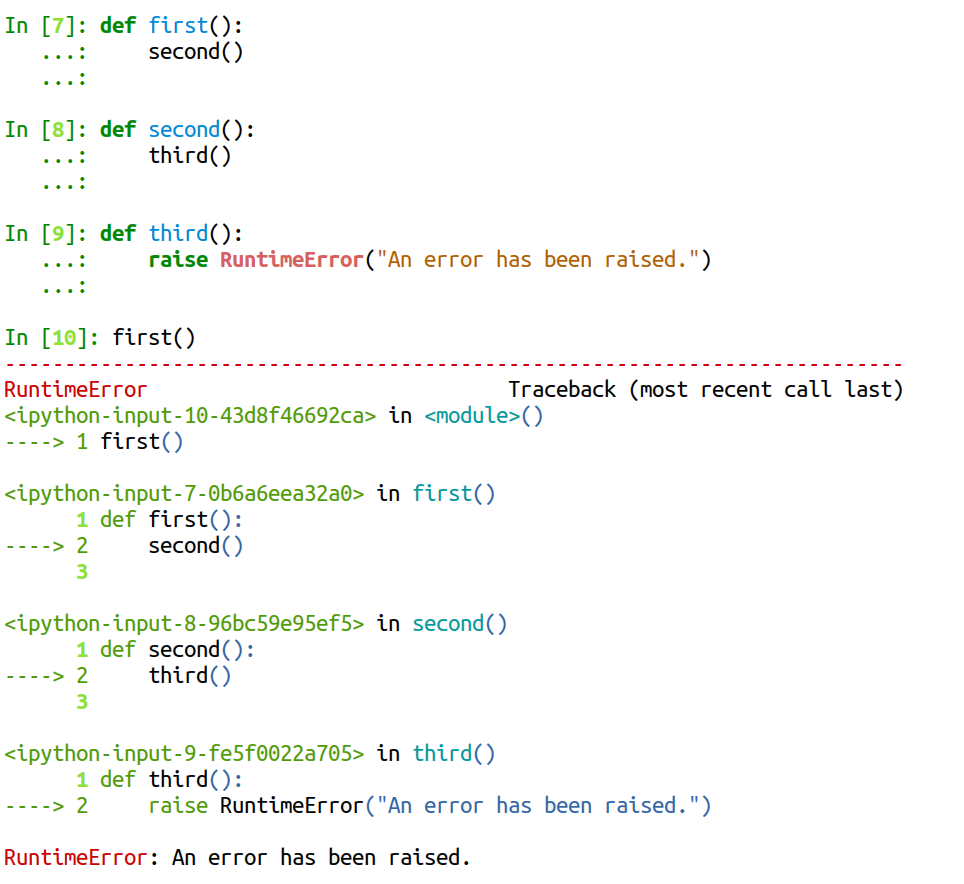
\includegraphics[width=.8\textwidth]{traceback.png}
    \caption{A traceback in an interactive shell with some dummy functions.}
    \label{traceback}
\end{figure}

\begin{figure}[h]
    \centering
    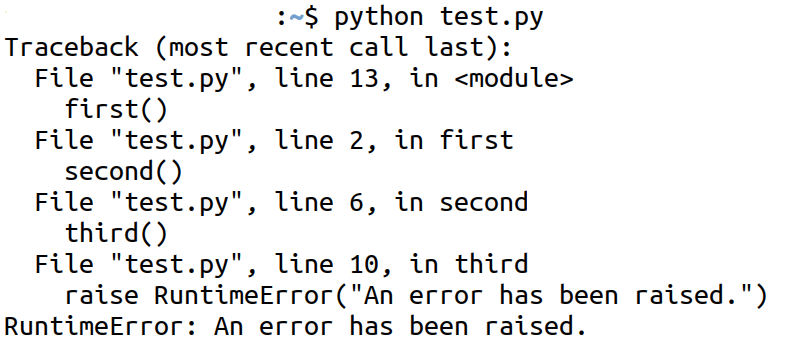
\includegraphics[width=.8\textwidth]{file-traceback.png}
    \caption{A traceback from the execution of a Python Script containing the functions from \ref{traceback}.}
    \label{file-traceback}
\end{figure}

\subsection{Debugger}



\section{Input and Output}

\href{http://pythontutor.com/visualize.html\#code=\%23\%20Opening\%20a\%20file\%20is\%20not\%20allowed\%20on\%20pythontutor.\%0A\%23\%20StringIO\%20gives\%20us\%20an\%20object\%0A\%23\%20that\%20behaves\%20like\%20a\%20file\%20handler.\%0Afrom\%20io\%20import\%20StringIO\%0A\%0Adef\%20message\%28file\%29\%3A\%0A\%20\%20\%20\%20if\%20file.closed\%3A\%0A\%20\%20\%20\%20\%20\%20\%20\%20print\%28\%22The\%20file\%20is\%20closed\%22\%29\%0A\%20\%20\%20\%20else\%3A\%0A\%20\%20\%20\%20\%20\%20\%20\%20print\%28\%22The\%20file\%20is\%20open.\%22\%29\%0A\%0A\%0A\%23\%20with\%20open\%28\%22filename\%22,\%20\%22r\%22\%29\%20as\%20file\%3A\%0Awith\%20StringIO\%28\%22Fake\%20file\%20content.\%22\%29\%20as\%20file\%3A\%0A\%20\%20\%20\%20message\%28file\%29\%0A\%20\%20\%20\%20print\%28file.read\%28\%29\%29\%0A\%20\%20\%20\%20print\%28file.read\%28\%29\%29\%0A\%20\%20\%20\%20file.seek\%280\%29\%0A\%20\%20\%20\%20print\%28file.read\%28\%29\%29\%0A\%0Amessage\%28file\%29\&cumulative=false\&curInstr=17\&heapPrimitives=nevernest\&mode=display\&origin=opt-frontend.js\&py=3\&rawInputLstJSON=\%5B\%5D\&textReferences=false}{Example for file reading.}

\section{Modules and Packages}
\section{Scope}
\section{Processing Data Formats}


\printbibliography[type=book,title={Book Sources}]

\end{document}
